\documentclass[notitlepage]{report}

\usepackage{titling}
\usepackage{blindtext}
\usepackage{amsmath}
\usepackage{amsthm}
\usepackage{amssymb}
\usepackage{float}
\usepackage{graphicx}
\usepackage{subfig}
\usepackage[utf8]{inputenc}
\usepackage[english]{babel}

\newtheorem{theorem}{Theorem}

\theoremstyle{definition}
\newtheorem{definition}{Definition}[section]

\title{%
	Collectives of local decision makers\\
	\large Construction Of A Boundary Hunter
}
\author{Daniel Braithwaite\\[1cm] {Supervisor: Marcus Frean}}

\begin{document}

\begin{titlingpage}
    \maketitle
    \begin{abstract}
    	Training a Multi Layer Perceptron (MLP) Network to solve supervised learning problems is common practice. When a problem is composed of subtasks then using an MLP Network has poor learning. The paper Adaptive Mixtures of Local Experts \cite{jacobs1991adaptive} proposes a Mixture of Experts model to solve this which is used in practice. This report speculates that decoupling the expert networks will further improve learning. The model developed in this paper allows experts to be dynamically trained and added as needed, it is able to perform well in low dimensions but encounters problems with learning as the number grows.
    \end{abstract}
\end{titlingpage}

\chapter{Introduction}

If Backpropagation is used to train a single Multi-Layer Network to peform distinct subtasks (parts of the data are generated by different sources) on diferent ocations, usially there will be inteference effects that can lead to slow convergence and poor generalization \cite{jacobs1991adaptive}.  In the paper Adaptive Mixtures of Local Experts \cite{jacobs1991adaptive} an idea was proposed to create a model where a number of Neural Netwroks (NN's), called experts, where trained on a subset of the data. Another NN called a gate is trained to assign examples to the experts. The gate takes examples and outputs the responsibility for each of the experts. Such a system is called a Mixtures of Experts (MoE) model. Such a model is called a Mixture of Experts (MoE). If a case is presented to a MoE model which it gets wrong then the weight changes are localized to the gating network and the networks to which it assigned the example. Therefore experts which operate in different situations (regions of the data) do not directly interfere with each others weights, significantly decreasing the dependency between expert networks.\\

In a MoE model with $n$ experts, when presented with an example to find the responsibilitys the gate outputs $x_1, ..., x_n$, the $x$'s are subsequently operated on by the softmax function, giving $p_j$, the responsibility expert $j$ has for the example, to be $p_j = \frac{e^{x_j}}{\sum_{i=1}^n e^{x_i}}$. \\

The MoE model can be thought of as a stocastic generator of vectors \cite{jacobs1991adaptive}. The responsibility $p_j$ can be thought of as the probability that the gating network picks expert $j$ as the output and the weights of each expert thought of as the mean of a gussian distrubution. Consequently the output of an MoE model can be thought of as first deciding on an expert and then choosing which a vector from the chosen experts gussian distrubution. The probability of expert $j$ being picked an generating output $o^c$ is given by equation \ref{equ:prob-exprtj-outoc}

\begin{align}
p_je^{-\frac{1}{2} \lVert \mu_j - o^c \lVert^2}
\label{equ:prob-exprtj-outoc}
\end{align}

It is known that the $p_j$'s sum to 1, so the probability of the MoE outputting $o^c$ is given by equation \ref{equ:prob-outc}

\begin{align}
P_{o^c} = \sum_{i=1}^n p_ie^{-\frac{1}{2} \lVert \mu_i - o^c \lVert^2}
\label{equ:prob-outc}
\end{align}

Equation \ref{equ:moe-loss} is the loss of an MoE, it is the negative log probability of generating the example based on the mixture of gussians model dicussed.

\begin{align}
E^c = -log \sum_{i=1}^n p^c_i e^{-\frac{1}{2} \lVert d^c - o_i^c \rVert^2 }
\label{equ:moe-loss}
\end{align}

Consider the partal deritive given in equation \ref{equ:moe-error-partial}

\begin{align}
\frac{\partial E^c}{\partial o_i^c} &= \bigg[ \frac{p_i^c e^{-\frac{1}{2} \lVert d^c - o_i^c \rVert^2}}{\sum_j p_j^c e^{-\frac{1}{2} \lVert d^c - o_j^c \rVert^2}} \bigg] \cdot (d^c - o_i^c)
\label{equ:moe-error-partial}
\end{align}

The term $\bigg[ \frac{p_i^c e^{-\frac{1}{2} \lVert d^c - o_i^c \rVert^2}}{\sum_j p_j^c e^{-\frac{1}{2} \lVert d^c - o_j^c \rVert^2}} \bigg]$ is a Softmax function on the output of our expert networks. Consequently we see that $\frac{\partial E^c}{\partial o_i^c}$ takes into account network $i$'s performance against all others, demonstrating that there is still dependency between the experts.\\

We speculate that further reducing the dependency between expert networks will improve learning. To motivate this problems with the MoE model are identified and it is explained how reducing dependency could solve them.\\ 

Currently if using an MoE model the number of experts must be decided beforehand. Requiring either prior knowledge about the number of subtasks in the problem or a trial and error process to find the optimal number. If the experts where completely independent then we could build our system sequentially by adding each one until we achieve our desired accuracy.\\

Consider a MoE model with only one expert. This will just act like a standard Perceptron Network, given the gate will assign all examples to the single expert, demonstrated by $p_1 = \frac{e^{x_1}}{\sum_i e^{x_i}} = \frac{e^{x_1}}{e^{x_1}} = 1$. Figure \ref{fig:intro-concrete-example} is a concrete example of how this results in a poor classifier which does not truly model the data. 

\begin{figure}[H]
	\centering
	\begin{minipage}[b]{0.5\textwidth}
		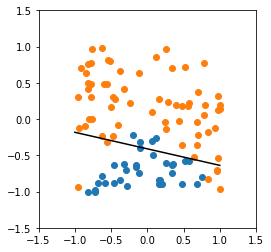
\includegraphics[width=\textwidth]{Standard-Perceptron.png}
		\caption{Example data for situation with line representing a trained perceptron}
		\label{fig:intro-concrete-example}
	\end{minipage}
	\hfill
\end{figure}

Shown in Fig \ref{fig:intro-concrete-example}, a single Perceptron (an MoE model with only one expert) trained on this data does not produce anything meaningful. The classifier achieves a low error but the decision boundary has not captured any structure of the data. If training a number of experts which have no dependency between one another then any update made to the weights of an expert  is only based off only its loss against the entire data set. The experts cant relie on others to classify things correctly, indiviually they must decide what they are or are not interested in. With no communication between experts could end up with some learning the same information. Perhaps the minimal amount of communication between experts needed is that they stay out of each others way.\\

In the current MoE model the dependency between experts is a consequence of two things, the gating network and that the error is a combination of the output from all experts. To remove this dependency each expert should decide what it is responsible for, thus making it possible to train them separately using an error function which only considers their individual outputs. \\

To investigate this speculation, we developed a model based on the previous observations. Experts are trained independently without any comuinication. Because of this experts can be added or removed from model as requried. These independent experts will be called \text{boundary hunters}\\

This paper reports on the development of our model and describes the path we followed to arrive at our final solution.

\chapter{Neuron Parametrisation}
A perceptron is learning a hyperplane called a decision boundary, defined by vector $w = [w_1, ..., w_n]$ normal to the hyperplane and a bias $b$ which shifts the decision boundary from the origin.

\theoremstyle{definition}
\begin{definition}
	A \text{Perceptron} with vector $w = [w_1, ..., w_n]$ normal to the decision boundary and bias $b$ has weighted sum for input $x = [x_1, ..., x_n]$ defined as
	
	\begin{align*}
		z = \sum_{i=1}^{n} w_i x_i
	\end{align*}
	
	and output $a(z) = f(z)$
	
	where $f(z) = 1$ indicates that $x$ is of class 1 and $f(x) = 0$ class 0.
\end{definition}

To define the boundary hunter it is necessary to be able to specify a region of interest, as discussed previously it must be able to decide what examples it is interested in. A logical way to define this region is to give the perceptron a centre and specify a radius around it, anything inside this area it will care about. A perceptron's parameters wont allow this, so the parametrisation must be adapted.

\section{Normal \& Point Parametrisation}
An equivalent definition for a perception can be formulated defined by a centre point and a hyperplane passing though it.

\theoremstyle{definition}
\begin{definition}
	The \textbf{Normal \& Point} parametrisation of a perceptron consists of the vector $w = [w_n, ..., w_n]$ normal to the hyperplane and $m = [m_n, ..., m_n]$ the point our hyperplane passes though.\\
	
	On input $x = [x_1, ..., x_k]$ the weighted sum is defined as 
	
	\begin{align*}
	z = \sum_{i=1}^n w_i \cdot (m_i - x_i)
	\end{align*}
	
	and output $a(z) = f(z)$
	
	where $f(z) = 1$ indicates that $x$ is of class 1 and $f(x) = 0$ class 0.
\end{definition}

\begin{theorem}
The normal \& point representation for a perceptron is equivalent to our standard definition
\end{theorem}

\begin{proof}
Assume that both parametrisations are using the same activation, then it is enough to show that the weighted sums would be the same. Let $w = [w_1, ..., w_n], m = [m_1, ..., m_n]$ be the parameters for a normal and point perceptron.

\begin{align*}
z &= \sum_{i=1}^n w_i \cdot (m_i - x_i)\\
&= w \cdot [m_1 - x_1, ..., m_n - x_n]\\
&= w_1 \cdot (m_1 - x_1) + ... + w_n \cdot (m_k - x_k)\\
&= w_1m_1 - w_1x_1 .... w_nm_k - w_nx_n\\
&= (w_1m_1 + ... + w_nm_n) - w_1x_1 - ... - w_nx_n
\end{align*}

Now an equivalent standard perceptron can be defined, with bias term $b = w_1m_1 + ... + w_nm_n$ and each component of the normal $m^{'}$ as $m^{'}_i = -m_i$.
\end{proof}

\subsubsection{Comparison To Perceptron}
Figures \ref{fig:com-standard-perceptron} \& \ref{fig:com-normal-point} compare the two parametrisations experimentally, confirming the proof presented above. Both converge to the same optimal solution. The centre of the normal and point perceptron is represented by the green dot in the graph.\\


\begin{figure}[H]
\centering
  \begin{minipage}[b]{0.4\textwidth}
    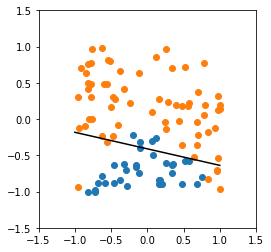
\includegraphics[width=\textwidth]{Standard-Perceptron.png}
    \caption{Standard Perceptron (SSE = 3.90)}
    \label{fig:com-standard-perceptron}
  \end{minipage}
  \hfill
  \begin{minipage}[b]{0.4\textwidth}
    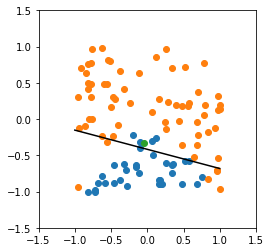
\includegraphics[width=\textwidth]{Modified-Perceptron-(Normal-Point).png}
    \caption{Modified Perceptron (SSE = 3.90)}
    \label{fig:com-normal-point}
  \end{minipage}
\end{figure}

\chapter{Boundary Hunter: First Attempt}
\section{Responsibility Function}
The \textbf{Normal \& Point Parametrization} has been shown to be equivalent to the regular Perceptron, it can now be used as a base to develop a boundary hunter. Before a suitable loss function can be designed the concept of responsibility must be further developed. Using the centre point plus a radius how can the boundary hunters responsibility for an example be quantified? Let $r$ be denoted the radius and $R(r, i)$ be the responsibility for example $i$.\\

A list of properties for $R$ follows.

\begin{enumerate}
	\item $R(r, i) \in [0, 1]$. This keeps the values constrained, a responsibility of 0 or 1 means we ether care or not retrospectively. This property also allows the "dont care" to be computed easiely, if $R(r, i)$ is how much the boundary hunter cares then $1 - R(r,i)$ is how much the boundary hunter does not care.
	\item $R(r, i)$ must continuous and differentiable so our gradients work with Backpropagation
	\item Any point inside or outside the area of interest should have responsibility close to 1 or 0 retrospectively. The radius is defining a caring region, anything inside it the boundary hunter cares about and anything outside it dosnt.
	\item Responsibility for points outside the area of interest should decrease as distance from area increases, this guarantees that as we move further away from the edge of our radius we get less interested
\end{enumerate}

A choice for $R$ is the logistic function, $f = 1 - \frac{1}{1 + e^{-S(x - x_0)}}$ where S is the steepness. $f$ meets requirements (1) - (4). The steepness can be thought of this as how rapidly our interest changes at the border of our region, a steep function means we rapidly move from caring to ignoring an example, where as a more gradual slope means it takes longer for us to loose interest.\\

The sigmoid function guarantees that any example will have $R(r, i) > \frac{1}{2}$, $R(r, i) < \frac{1}{2}$, $R(r, i) = \frac{1}{2}$ if it is inside, outside or on the border retrospectively. As $S \rightarrow \infty$ then the responsibility approaches a step function, being 1 for any example inside the boundary hunters region and 0 otherwise. If the steepness is to low then examples far away from the boundary hunter will have to much of an impact, on the other hand if its to high then the boundary hunter wont consider any example its not interested in. From inspecting the graphs for various steepnesses, $S = 10$ is a goood place to start, the responsibility decays rappidly but slow enough to consider a range of points in/out side the area of interest.

\begin{align}
R(r, i) = 1 - \frac{1}{1 + e^{-10(d_i-r)}}
\label{equ:responsibility}
\end{align}

where $d_i$ is the distance example $i$ is from the boundary hunters centre.

\section{Loss Function Design: Attempt 1}
\label{sec:lossfunction-a1}
For an example $i$ let the output of a boundary hunter be denoted by $\widehat{t_i}$. $\widehat{t_i}$ is the probability that example $i$ has a class of 1, i.e. $p_{t_i=1} = \widehat{t_i}$ and $p_{t_i=0} = 1 - \widehat{t_i}$. If the true class is 1 then probability of being correct $p_c$ is $p_{t_i=1}$, likewise if the true class is 0 then $p_c = p_{t_i=0}$. $\widehat{t_i}$ can also be thought of as the certianty that example $i$ has class 1, so if $\widehat{t_i} = \frac{1}{2}$ then the boundary hunter is completly uncerten as to the class of the example. To develop this idea of the boundary hunters certenty consider if the given example has a high responsibility (i.e. is close to the boundary hunters centre) then the hunter should be certain its answer is correct, likewise a low responsibility means the example is far from the boundary hunters centre and therefore it should be uncertain about the correctness of its answer.\\

As uncertainty about the boundary hunters output increases $t_i$ (probability of the examples true class being 1) approaches $\frac{1}{2}$, a fair coin toss, i.e. $R(r, i) \rightarrow 0$ then $\widehat{t_i} \rightarrow \frac{1}{2}$.\\

If the boundary hunter has a high responsibility for an example then the error is its accuracy at predicting the correct class, using the cross entropy this is quantified as $t_i log(\widehat{t_i}) + (t_i)log(1 - \widehat{t_i})$. If the responsibility for an example is low then its penalty for that instance is the error for predicting a fair coin toss, also using the cross entropy results with $log(\frac{1}{2})$. Equation \ref{equ:loss1} is the resulting loss function

\begin{align}
L = -\frac{1}{N} \sum_{n=0}^N R(r, n) (t_n log(\widehat{t_n}) + (1-t_n)log(1 - \widehat{t_n})) + (1-R(r, n)) log(1/2)
\label{equ:loss1}
\end{align}

\subsection{Experimental Results}
Figure \ref{fig:boundaryhunter-l1-01} shows a boundary hunter trained with equations \ref{equ:responsibility} \& \ref{equ:loss1} for the loss and responsibility functions.

\begin{figure}[H]
\centering
  \begin{minipage}[b]{0.4\textwidth}
    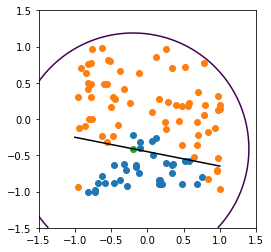
\includegraphics[width=\textwidth]{BoundaryHunter-Attempt1-01.png}
    \caption{Boundary Hunter with \ref{equ:loss1} as loss and \ref{equ:responsibility} as responsibility}
    \label{fig:boundaryhunter-l1-01}
  \end{minipage}
  \hfill
\end{figure}

The boundary hunter has learnt to care about all the data which is the opposite of learning to ignore sections of the data.

\subsection{Discussion}
Consider that the boundary hunter is a single neuron and consequently the partial deritive $\frac{\partial E}{\partial w_i}$ is given by

\begin{align}
\frac{\partial E}{\partial w_i} &= \lambda \frac{\partial E}{\partial \widehat{t}} \cdot \frac{\partial \widehat{t}}{\partial z} \cdot \frac{\partial z}{\partial w_i}
\end{align}

Equation \ref{equ:final-de-dw-l1} substutes in the derivitation of $\frac{\partial E}{\partial \widehat{t}}$ given in \ref{equ:de-dt-l1} 

\begin{equation}
\begin{aligned}
\frac{\partial E}{\partial \widehat{t}} &= \frac{\partial}{\partial \widehat{t}} \big[ R(r, j) \cdot (t \cdot \log(\widehat{t}) + (1-t)\cdot \log(1 - \widehat{t}) + (1-R(r,j)) \cdot \log(\frac{1}{2}) \big]\\
&= \frac{R(r, j) \cdot t}{\widehat{t}} + \frac{R(r, j) \cdot (1 - t)}{\widehat{t} - 1}\\
&= R(r, j) \cdot \frac{(t - \widehat{t})}{(\widehat{t} - 1) \widehat{t}}
\label{equ:de-dt-l1}
\end{aligned}
\end{equation}

\begin{equation}
\begin{aligned}
\frac{\partial E}{\partial w_i} &= \lambda \big[ R(r, j) \cdot \frac{(t - \widehat{t})}{(\widehat{t} - 1) \widehat{t}} \big] \cdot \frac{\partial \widehat{t}}{\partial z} \cdot \frac{\partial z}{\partial w_i}\\
&= \big[\lambda \cdot R(r,j) \big] \cdot \frac{(t - \widehat{t})}{(\widehat{t} - 1) \widehat{t}} \cdot \frac{\partial \widehat{t}}{\partial z} \cdot \frac{\partial z}{\partial w_i}
\label{equ:final-de-dw-l1}
\end{aligned}
\end{equation}

The equation \ref{equ:final-de-dw-l1} demonstraits why this loss function does not achieve the desired results. The responsibility becomes an multiplier on the learning rate, consequently the boundary hunter is optimizing the standard cross entropy loss. The same can be shown for the gradients $\frac{\partial E}{\partial \partial m_i}$

Figure \ref{fig:boundaryhunter-l1-01} shows the boundary hunter has a high responsibility for every example, reducing \ref{equ:loss1} to the standard cross entropy loss

\begin{align*}
L = -\frac{1}{N} \sum_{n=0}^N R(r, n) (t_n log(\widehat{t_n}) + (1-t_n)log(1 - \widehat{t_n}))
\end{align*} 

The solution which the boundary hunter converged on allows miss classifications, indicating that the penalty for taking a guess and getting it wrong is to low.

\section{Loss Function Design: Attempt 2}
Consider the boundary hunter as a salesperson, who gets paid $\$B$ for selling something to someone who wants it (if the salesperson is responsible for this individual) and gets penalized $\$C$ dollars for selling something to someone who does not want it. Using this model, the salesperson is to position them selves and adjust their responsibility so that they are maximizing there profit.\\

$y^t(1-y)^{t-1}$, $y^{t-1}(1-y)^t$ is the probability the boundary hunter outputs a correct or wrong classification retrospectively, consequently giving equation \ref{equ:loss2} as a candidate loss function for a boundary hunter.

\begin{align}
L = \sum_{i=0} R(r, i) * \big[Cy_i^{1-t_i}(1-y_i)^{t_i} - By_i^{t_i}(1-y_i)^{1-t_i} \big]
\label{equ:loss2}
\end{align}

\subsection{Experimental Results}
Figure \ref{fig:boundaryhunter-l2-01} shows the result of training a boundary hunter with equations \ref{equ:loss2} \& \ref{equ:responsibility} as the loss and responsibility functions. With a similar solution to using equation \ref{equ:loss1} as the loss function the boundary hunter includes every example in its area of interest.\\

\begin{figure}[H]
\centering
  \begin{minipage}[b]{0.4\textwidth}
    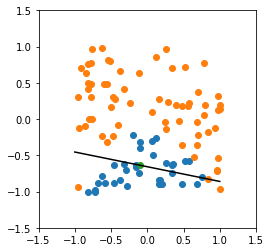
\includegraphics[width=\textwidth]{BoundaryHunter-Attempt3-01.png}
    \caption{Boundary Hunter with (3.5) as loss and (3.2) as responsibility}
    \label{fig:boundaryhunter-l2-01}
  \end{minipage}
  \hfill
\end{figure}

The cost of miss classifying a few examples is outweighed by the reward of getting all other examples correct. This demonstrates that the parameter C (cost for incorrect classification) is to low. It is unclear the extent to which increasing C will change the optimal solutions, to get a good spread 1.3, 1.6, 1.9 are used as values for C

\begin{figure}[H]
  \centering
  \begin{minipage}[b]{0.49\textwidth}
    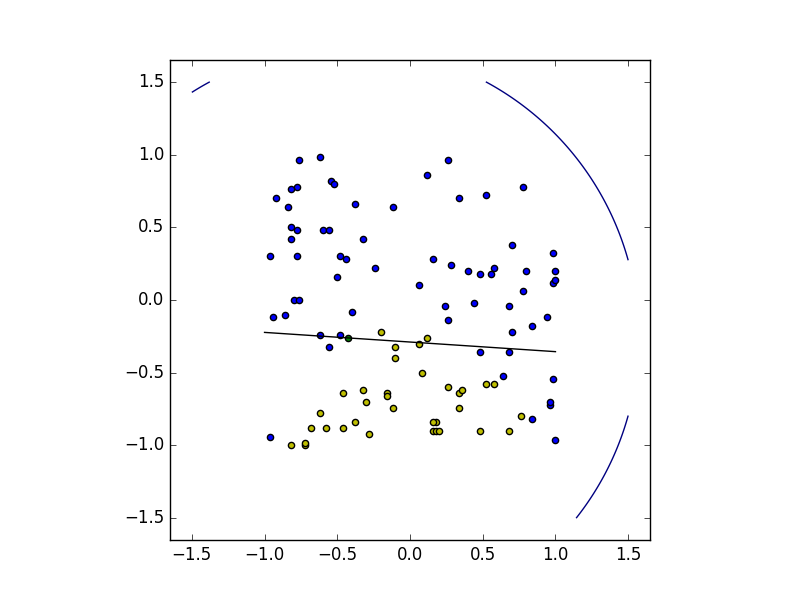
\includegraphics[width=\textwidth]{BoundaryHunter-Attempt3-02.png}
    \caption{C = 1.3}
    \label{fig:boundaryhunter-l2-02}
  \end{minipage}
  \hfill
  \begin{minipage}[b]{0.49\textwidth}
    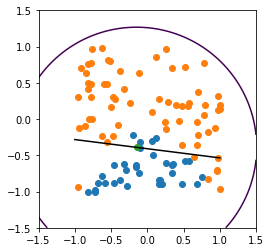
\includegraphics[width=\textwidth]{BoundaryHunter-Attempt3-03.png}
    \caption{C = 1.6}
    \label{fig:boundaryhunter-l2-03}
  \end{minipage}
  \hfill
  \begin{minipage}[b]{0.49\textwidth}
    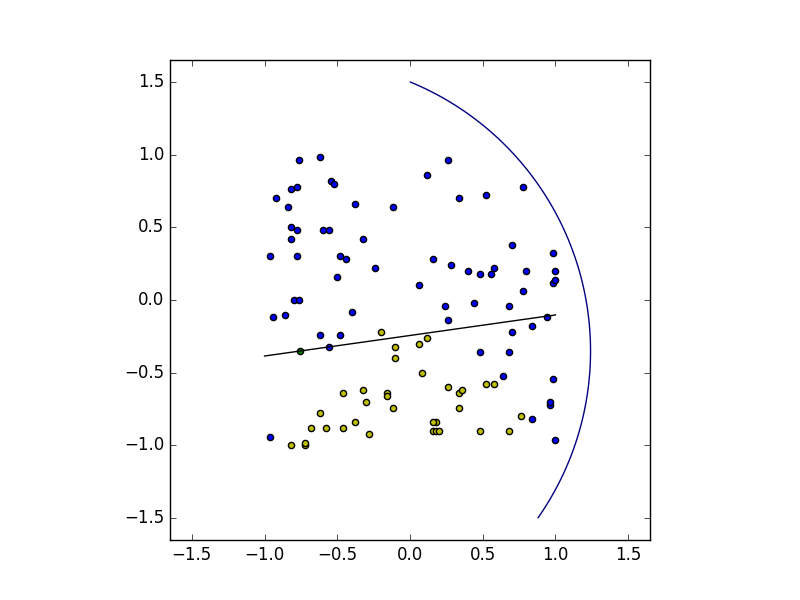
\includegraphics[width=\textwidth]{BoundaryHunter-Attempt3-04.png}
    \caption{C = 1.9}
    \label{fig:boundaryhunter-l2-04}
  \end{minipage}
\end{figure}

Figures \ref{fig:boundaryhunter-l2-02}, \ref{fig:boundaryhunter-l2-03} \& \ref{fig:boundaryhunter-l2-04} show that this only changes the hyperplane positioning, it does not stop the boundary hunter from being interested in all examples. If some reasonable restrictions are imposed on the radius (i.e. $0.3 \leq r \leq 0.8$), set C = 1.9 and adjust the responsibility function to be less steep (steepness of 5) then some better results are achieved, which are more in line with the goal.

\begin{figure}[H]
  \centering
  \begin{minipage}[b]{0.4\textwidth}
    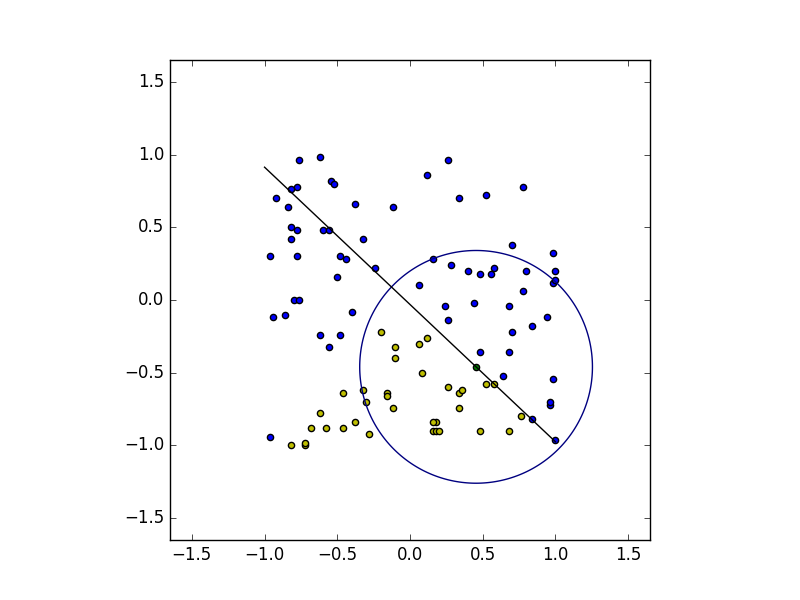
\includegraphics[width=\textwidth]{BoundaryHunter-Attempt3-R0.png}
    \caption{}
    \label{fig:boundaryhunter-l2-good1}
  \end{minipage}
  \hfill
  \begin{minipage}[b]{0.4\textwidth}
    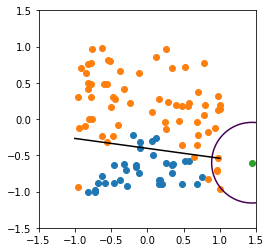
\includegraphics[width=\textwidth]{BoundaryHunter-Attempt3-R1.png}
    \caption{}
    \label{fig:boundaryhunter-l2-good2}
  \end{minipage}
  \hfill
\end{figure}

More often than not the boundary hunter converges on a solution like the one shown in figure \ref{fig:boundaryhunter-l2-badresults}, these do not achieve anything meaningful as the solution is to classify almost all points as a singular class.

\begin{figure}[H]
  \centering
  \begin{minipage}[b]{0.5\textwidth}
    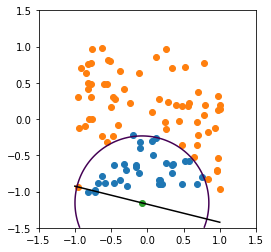
\includegraphics[width=\textwidth]{BoundaryHunter-Attempt3-R2.png}
    \caption{}
    \label{fig:boundaryhunter-l2-badresults}
  \end{minipage}
  \hfill
\end{figure}

The solutions shown in figures \ref{fig:boundaryhunter-l2-good1} \& \ref{fig:boundaryhunter-l2-good2} by inspection have lower error than figure \ref{fig:boundaryhunter-l2-badresults}, consequently the issue we are observing must be that of local optima.\\

The local optima become visible in figures \ref{fig:lossplot-01}, \ref{fig:lossplot-02} \& \ref{fig:lossplot-03}. These plots show the loss for each possible centre position of the boundary hunter. The hyperplane has been fixed so that it aligns with the left side of the chevron. The responsibility has a steepness of 5 and C = 1.9.

\begin{figure}[H]
  \centering
  \begin{minipage}[b]{0.8\textwidth}
    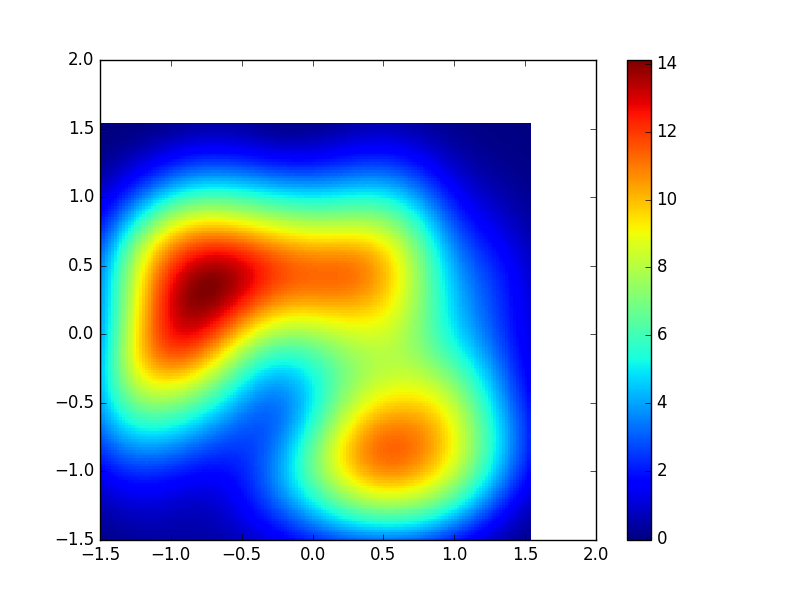
\includegraphics[width=\textwidth]{LossPlot-1.png}
    \caption{Radius as 0.3}
    \label{fig:lossplot-01}
  \end{minipage}
  \hfill
\end{figure}

\begin{figure}[H]
  \centering
  \begin{minipage}[b]{0.8\textwidth}
    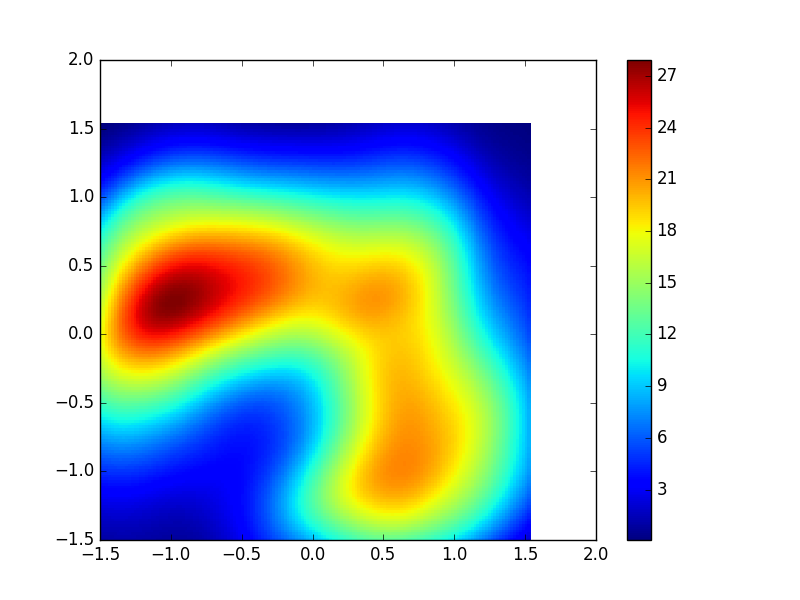
\includegraphics[width=\textwidth]{LossPlot-2.png}
    \caption{Radius as 0.8}
    \label{fig:lossplot-02}
  \end{minipage}
  \hfill
\end{figure}

\begin{figure}[H]
  \centering
  \begin{minipage}[b]{0.8\textwidth}
    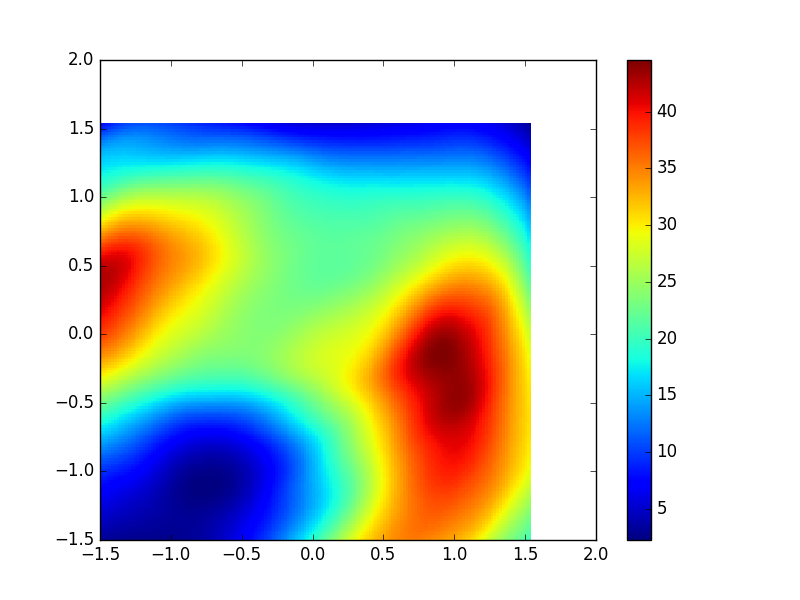
\includegraphics[width=\textwidth]{LossPlot-3.png}
    \caption{Radius as 2.0}
    \label{fig:lossplot-03}
  \end{minipage}
  \hfill
\end{figure}

Figures \ref{fig:lossplot-01}, \ref{fig:lossplot-02} \& \ref{fig:lossplot-03} show that while there is an optima aligned with the left side of the chevron there are more optima at the edges of the examples, corresponding to figure \ref{fig:boundaryhunter-l2-badresults}

Outside the boundary hunter's area of interest the responsibility for any example rapidly approaches 0 as the distance from the centre increases. As the boundary hunter moves away from all examples thus excluding all from its interest then error approaches 0. This seems to indicate that the responsibility function is to steep because the boundary hunter does not care enough about examples outside its interest.

\begin{figure}[H]
  \centering
  \begin{minipage}[b]{0.8\textwidth}
    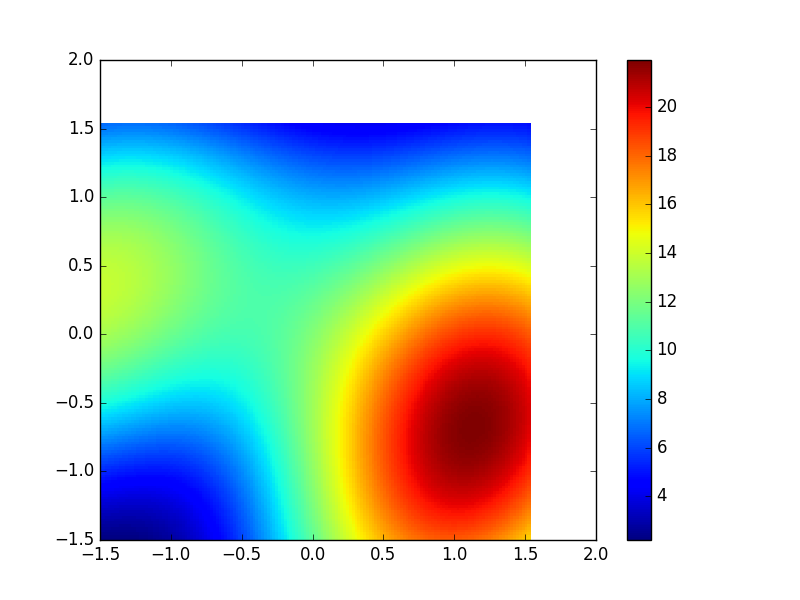
\includegraphics[width=\textwidth]{LossPlot-4.png}
    \caption{Radius as 0.3, with steepness as 0.5}
    \label{fig:lossplot-04}
  \end{minipage}
  \hfill
\end{figure}


Figure \ref{fig:lossplot-04} demonstrates that even with a less steep responsibility function the same local optima issues exists. 

\section{Discussion}
Based on these findings this reports concludes that trying to incorporate the responsibility into a loss function is, in essence a careful balancing act of rewards and penalty's for which there is possibly no solution. Consequently a new approach is needed.

\chapter{Radial Basis Function Networks}
Radial Basis Function (RBF) Networks seem closely related to a boundary hunter. Before this connection can be made a brief overview of RBF Networks will be given by first defining an RBF Function.\\

\theoremstyle{definition}
\begin{definition}
	If $f$ is an \textbf{Radial Basis Function} then its output depends only on the distance from its input to some point $c$, called the centre of $f$.
	
	\begin{align}
		f(x, c) = g(\lVert x - c \lVert)
	\end{align}
\end{definition}

\theoremstyle{definition}
\begin{definition}
	A \textbf{Radial Bias Function Neuron} has activation $a$ which is an RBF with centre $c$. On input x the output of an RBF Neuron is $a(x, c)$
\end{definition}

\theoremstyle{definition}
\begin{definition}
	A \textbf{Radial Bias Function Network} consists of three layers, input, hidden and output. The hidden layer consists of \text{Radial Bias Function Neurons}. There are no weights between the input and hidden layers, the example given to the RBF Network is passed directly to the RBF Neurons. The output layer consists of standard perceptrons.
\end{definition}

Each RBF Neuron is measuring the similarity between its centre and the input vector presented to it, the closer the input is to the centre the closer the activation is to 1. Any RBF is sutible to be an activation, a commonly used one is based off the 1D Gussian

\begin{align*}
f(x) = \frac{1}{\sigma \sqrt{2 \pi}} e^{-\frac{(x-\mu)^2}{2\sigma^2}}
\end{align*}

Which can be simplified to give

\begin{align}
a(x) = e^{-\beta \lVert x - c \lVert^2}
\end{align}

We use the $\beta$ term to control how quickly the activation decays.\\

An intuitive view of an RBF Network is a number of RBF Neurons measure how similar a given input vector is to their centre, which gets reported to the output neurons. Each output neuron then use this information to make a decision about their activation by taking a weighted sum of the outputs from the RBF Neurons.\\

\section{Training RBF Networks}
The simplest method for training RBF Networks is to randomly initialize all parameters in
 the network and use gradient descent to optimize them.

\begin{figure}[H]
  \centering
  \begin{minipage}[b]{0.7\textwidth}
    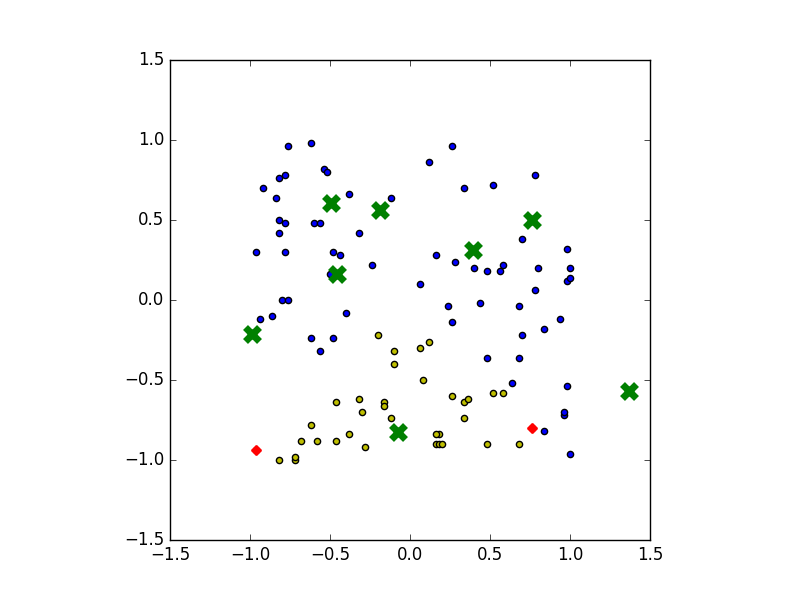
\includegraphics[width=\textwidth]{RBFN-01.png}
    \caption{}
    \label{fig:RBFN-01}
  \end{minipage}
  \hfill
\end{figure}
\begin{figure}[H]
  \centering
  \begin{minipage}[b]{0.7\textwidth}
    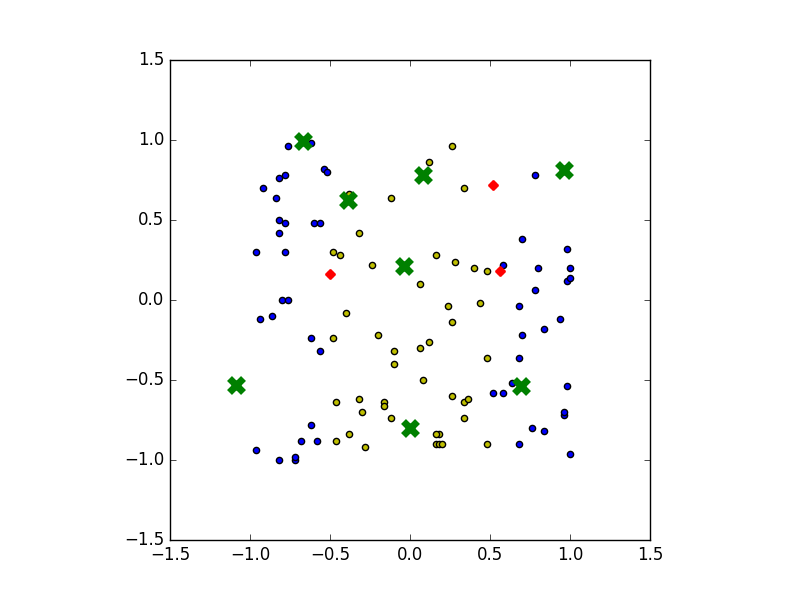
\includegraphics[width=\textwidth]{RBFN-02.png}
    \caption{}
    \label{fig:RBFN-02}
  \end{minipage}
  \hfill
\end{figure}
\begin{figure}[H]
  \centering
  \begin{minipage}[b]{0.7\textwidth}
    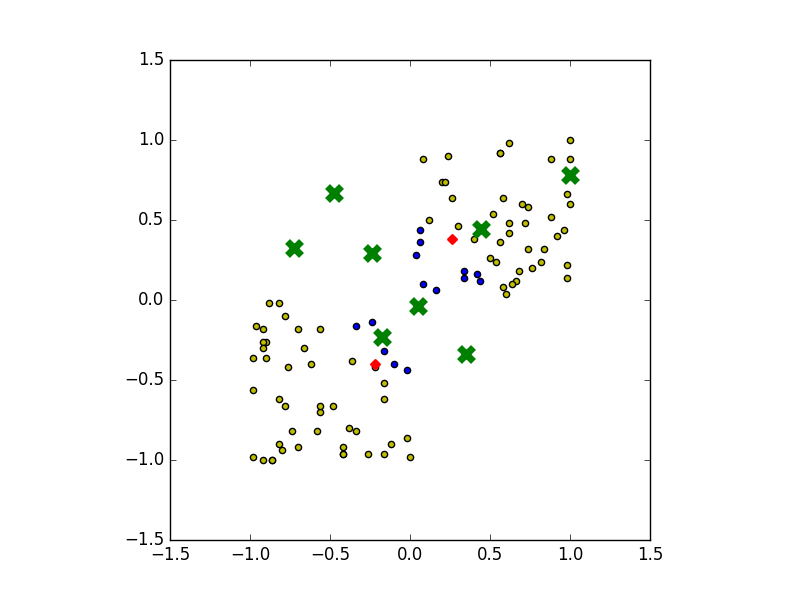
\includegraphics[width=\textwidth]{RBFN-03.png}
    \caption{}
    \label{fig:RBFN-03}
  \end{minipage}
  \hfill

The green x's and red x's represent our centroids and the points we are getting incorrect retrospectively
\end{figure}

Figures \ref{fig:RBFN-01}, \ref{fig:RBFN-02} and \ref{fig:RBFN-03} show RBF Networks trained over three different data sets. In each case the overall classifier has achieved a good model for the data, only getting a few examples wrong in each case.\\

\section{Discussion}
RBF Neurons do not make any decisions about the data, they only report on the similarity between the input vector and their centre. Consider the activation of an RBF Neuron as the certainty that the neuron is responsible about an example, a closer example means a higher certainty about responsibility. Now the output of an RBF Network can be thought of as a decision based off number of certainties about a given examples position.\\

This is what a boundary hunter should be doing, except instead of reporting the certainty of responsibility it will output its certainty of the examples class.

\chapter{RBF Based Boundary Hunters}
Based on these RBF Networks, is it possible to construct a boundary hunter? In this chapter an activation function for an RBF Boundary Hunter Neuron is derived.\\

Consider that the output of an RBF Neuron is the uncertainty about whether it is responsible for the given example, as the point gets further away the neuron becomes less certain about our ownership and so the activation decreases in value. In the case of an RBF Boundary Hunter its activation reflects the neurons certainty of the examples class, as the distance from the boundary hunters centre increases then the neuron will be less certain of its classification.\\

Let $f$ be the activation function for an RBF Boundary Hunter. As the belief that the example has a class of 1 increases $f \rightarrow 1$ and as the belief decreases $f \rightarrow 0$, so if $f = \frac{1}{2}$ then the neuron is completely uncertain about the classification. Consequently as the distance between the boundary hunter's centre and an example increases $f \rightarrow \frac{1}{2}$. The definition of an RBF Boundary Hunter can now be given.\\

\theoremstyle{definition}
\begin{definition}
A \textbf{RBF Boundary Hunter Neuron} (for binary classification) in $\mathbb{R}^n$ has $2n + 1$ free parameters. $\beta \in \mathbb{R}$, $\mathbf{c} \in \mathbb{R}^n$ and $\mathbf{n} \in \mathbb{R}^n$. $\beta, \mathbf{c}$ represent decay speed and centre of the RBF portion of our neuron. $\mathbf{n}$ defines a hyperplane which passes through our point $\mathbf{c}$. We define the activation as follows

\begin{align}
a(x) &= \frac{1}{2} + e^{-\beta \lVert x - c \lVert^2}(\frac{1}{1 + e^{-(\mathbf{n} \cdot (\mathbf{c} - x))}} - \frac{1}{2})
\label{equ:rbf-bh-activation}
\end{align}

\end{definition}

\subsection{Training RBF Boundary Hunters}
Using the same method as before, randomly initializing all parameters and then training using gradient descent.

In figures \ref{fig:RBFN-BH-01}, \ref{fig:RBFN-BH-02} and \ref{fig:RBFN-BH-03} green x's represent the centroids while the red x's the incorrect classifications.


\begin{figure}[H]
  \centering
  \begin{minipage}[b]{0.7\textwidth}
    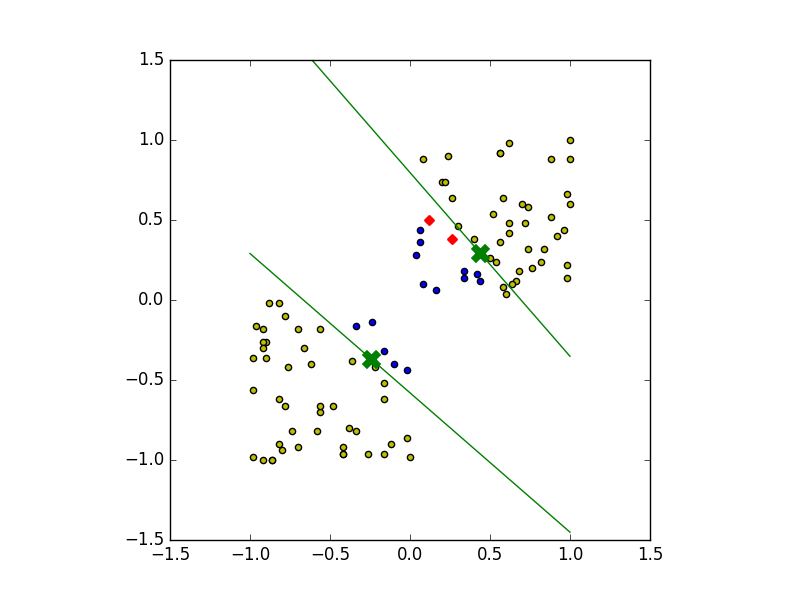
\includegraphics[width=\textwidth]{RBFN-BH-01.png}
    \caption{}
    \label{fig:RBFN-BH-01}
  \end{minipage}
  \hfill
\end{figure}
\begin{figure}[H]
  \centering
  \begin{minipage}[b]{0.7\textwidth}
    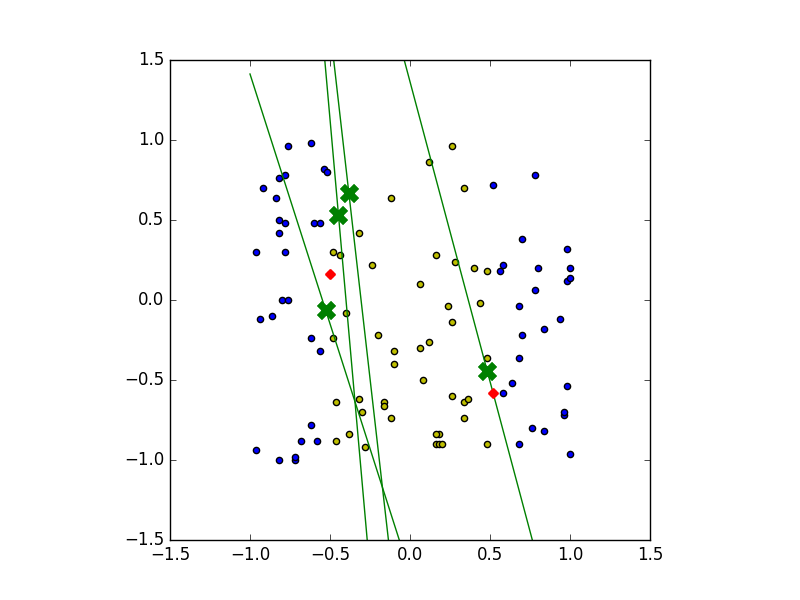
\includegraphics[width=\textwidth]{RBFN-BH-02.png}
    \caption{}
    \label{fig:RBFN-BH-02}
  \end{minipage}
  \hfill
\end{figure}
\begin{figure}[H]
  \centering
  \begin{minipage}[b]{0.7\textwidth}
    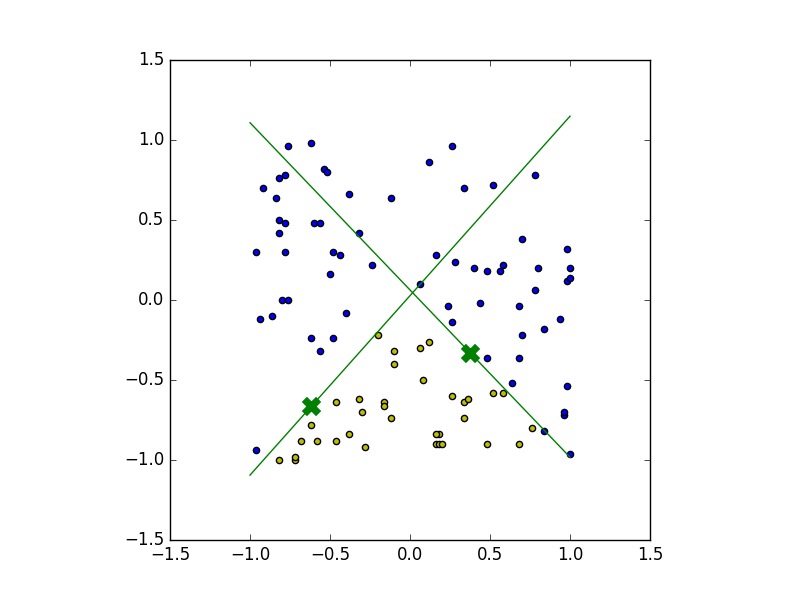
\includegraphics[width=\textwidth]{RBFN-BH-03.png}
    \caption{}
    \label{fig:RBFN-BH-03}
  \end{minipage}
  \hfill
\end{figure}

The hyperplanes are certainly being placed on boundaries in the data. Returning to the motivation for this project, what happens if a single RBF Boundary Hunter neuron is trained on the chevron data set?

\begin{figure}[H]
  \centering
  \begin{minipage}[b]{0.7\textwidth}
    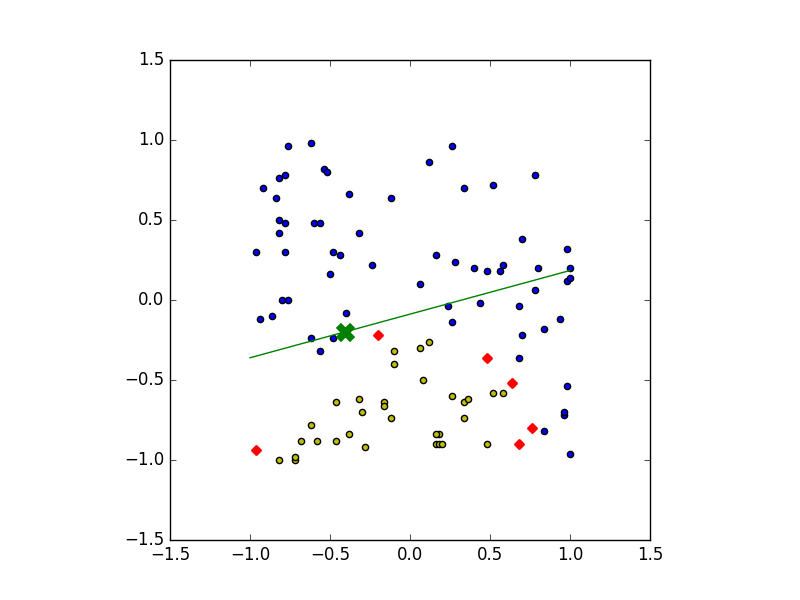
\includegraphics[width=\textwidth]{RBFN-BH-04.png}
    \caption{}
    \label{fig:RBFN-BH-04}
  \end{minipage}
  \hfill
\end{figure}

Figure \ref{fig:RBFN-BH-04} demonstrates that these RBF Boundary Hunter Networks still suffer from dependency between the neurons. If there was no dependency between the boundary hunters then the hyperplane in figure \ref{fig:RBFN-BH-04} would be one of the planes shown in \ref{fig:RBFN-BH-03}, seeing as this is not the case then the two boundary hunters must be dependent on each other.

\section{Gated Neurons}
Moving away from the idea of RFB Neurons and generalizing the concept of a RBF Boundary Hunter Neuron to what will be called a \textbf{Gated Neuron}. This will allow different methods to be defined for computing the responsibility.

\theoremstyle{definition}
\begin{definition}
A \textbf{Gated Neuron} consists of two functions, a \textbf{gating function} $g$ and prediction function $f$. $g$ takes the neurons input and outputs our certainty about the classification for that point, if $g$ is 0 then the neuron is completely unsure about the input and if $g$ is 1 then it is certain. The Gated Neuron activation function is defined below

\begin{align}
a(x) &= \sigma(g(x) \cdot f(x))
\label{equ:gated-neuron-activation}
\end{align}

\textbf{Note: } Equation \ref{equ:gated-neuron-activation} is not equivalent to our previous activation \ref{equ:rbf-bh-activation}. The gating operation has been moved inside the sigmoid function as this is simpler.

\end{definition}

Then a Gated Neuron (GN) Network is a feed-foward network where the hidden neurons are Gated Neurons.

\section{Hyperplane Gated Neuron}
A hyperplane gated neuron can now be defined, the neuron has a second hyperplane which is used to divide the space into two parts, the ones its responsible for and the ones it is not. In a similar fashion to before this definition will include a centre point.

\theoremstyle{definition}
\begin{definition}
A \textbf{Hyperplane Gated Neuron} is a gated neuron with the following parameters and functions. A centre point $c$ and two hyperplanes $n$ and $m$ passing through $c$. $n$ is normal to the decision boundary and $m$ is normal to a hyperplane which divides the plane into parts, the do and don't care sections. Therefore giving $g = \sigma(m \cdot (c - x))$ and $f = n \cdot (c - x)$. The resulting activation function is

\begin{align}
a(x) = \sigma(\sigma(m \cdot (c - x)) \cdot (n \cdot (c - x)))
\end{align}

\end{definition}

Which when in a GN Network and trained on the chevron data gives the following result

\begin{figure}[H]
  \centering
  \begin{minipage}[b]{0.7\textwidth}
    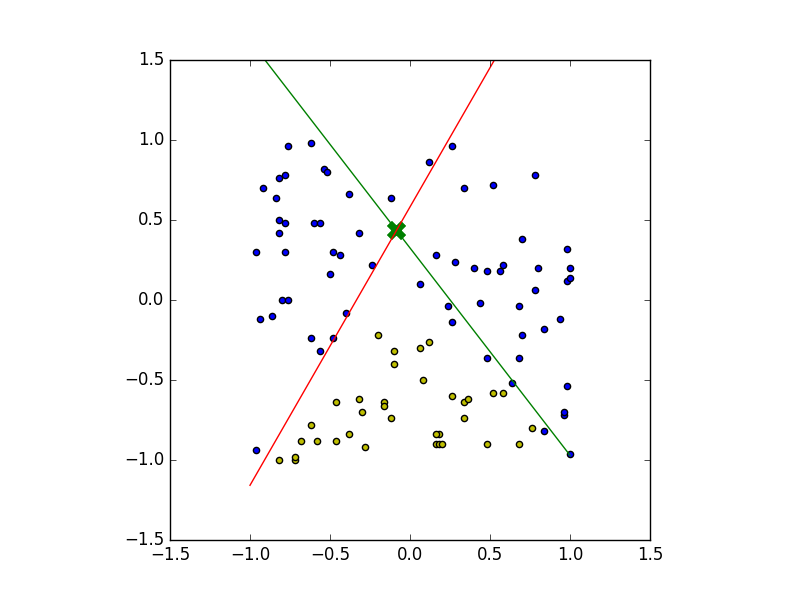
\includegraphics[width=\textwidth]{GN-MH-01.png}
    \caption{}
  \end{minipage}
  \hfill

The red line represents the gating hyperplane and the green line represents the decision boundary
\end{figure}

This is precisely what we are looking for in terms of classifying a chevron with only one boundary hunter.

\subsection{Comparison To Perceptron}
These boundary hunters have $3n$ free parameters, a little less than three times the number required for a regular perceptron, so a reasonable question to ask is what can be achieved with a three layer perceptron network?\\

Is it possible to achieve better performance with a standard Multi Layer Perceptron (MLP) Network containing 3 hidden neurons. This network configuration has been chosen as it contains a similar number of free parameters to the Hyperplane GN Network.

This comparison will be performed on the chevron dataset, using 10-Fold Cross Validation and computing a 95\% confidence interval on the accuracies.

\begin{center}
\begin{tabular}{| c | c | c |}
\hline
Network & Avg Training Error & Avg Test Error \\
\hline
\hline
Perceptron & 0.00749882335194 & 0.0172678373009 \\
\hline
Gated Neuron & 0.0244635285134 & 0.0354204954447 \\
\hline
\end{tabular}
\end{center}

\begin{center}
\begin{tabular}{| c | c | c |}
\hline
Network & Training Error Conf Interval & Avg Test Error Conf Interval\\
\hline
\hline
Perceptron & (0.007, 0.008) & (0.007, 0.028)\\
\hline
Gated Neuron & (0.014, 0.035) & (0.012, 0.059)\\
\hline
\end{tabular}
\end{center}

These 95\% confidence intervals show that there is a statistically significant difference between the training but not the test accuracies, so it can be concluded that the two methods have the same performance.

\subsection{Redundancy}
The definition of a Hyperplane Gated Neuron included a centre point, which is redundant. The point is specifying the intersection of our two lines which this is not needed. Figure \ref{fig:GN_MH-ONLY-01} demonstrates that this point can be removed and the same results can be achieved but with fewer free parameters, only 2n + 2 to be precise.

\begin{figure}[H]
  \centering
  \begin{minipage}[b]{0.8\textwidth}
    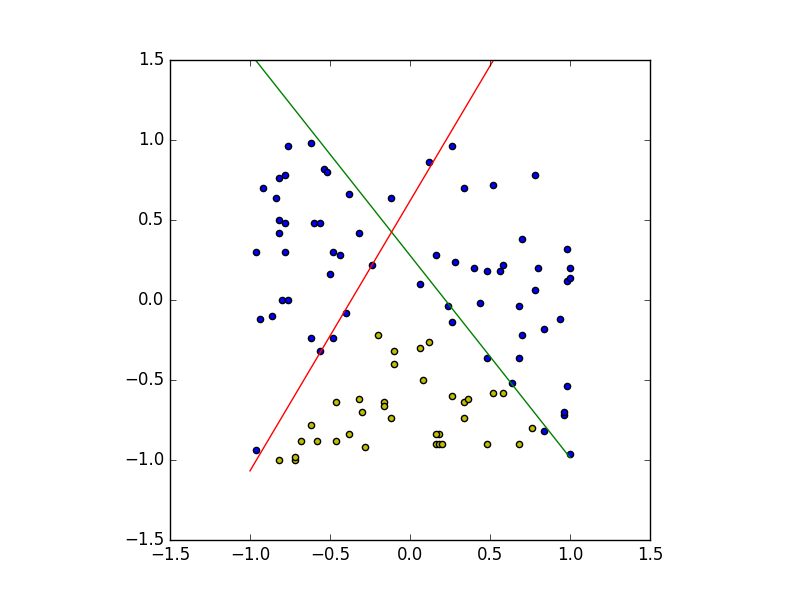
\includegraphics[width=\textwidth]{GN-MH-ONLY-01.png}
    \caption{}
    \label{fig:GN_MH-ONLY-01}
  \end{minipage}
  \hfill

Hyperplane Gated Boundary Hunter without the centre point
\end{figure}

Comparing the performance of these new hyperplane gated boundary hunters against a standard perceptron network with 2 hidden neurons gives the following.

\begin{center}
\begin{tabular}{| c | c | c |}
\hline
Network & Avg Training Error & Avg Test Error \\
\hline
\hline
Perceptron & 0.023 & 0.037 \\
\hline
Gated Neuron & 0.023 & 0.031 \\
\hline
\end{tabular}
\end{center}

\begin{center}
\begin{tabular}{| c | c | c |}
\hline
Network & Training Error Conf Interval & Avg Test Error Conf Interval\\
\hline
\hline
Perceptron & (0.010, 0.037) & (0.013, 0.061)\\
\hline
Gated Neuron & (0.017, 0.030) & (0.008, 0.053)\\
\hline
\end{tabular}
\end{center}

With this modification there is still no statistically significant difference between the performance of the two networks.

\subsection{Discussion}
Does this current solution solve the problem laid out at the beginning of this report. How is this solution different to the one proposed in Adaptive Mixtures of Experts \cite{jacobs1991adaptive}. The goal was to create neurons which act independently and learn to classify local features of the data.\\

Compared to the MoE model it would definitely appear that Hyperplane GN Networks have less dependency between the hidden neurons, each GN is responsible for deciding its interest which is not the case in the MoE model.\\

One thing to consider however is that a Hperlplane GN Network has an output layer, taking the classification from each of the boundary hunters and making the final decision about the examples class. The output layer reintroduces some dependency between the hidden neurons, demonstrated by figures \ref{fig:RecData-1HP} \& \ref{fig:RecData-2HP}.\\

In figure \ref{fig:RecData-1HP}, the single boundary is unable to identify any sides of the rectangle boundary.

\begin{figure}[H]
  \centering
  \begin{minipage}[b]{0.8\textwidth}
    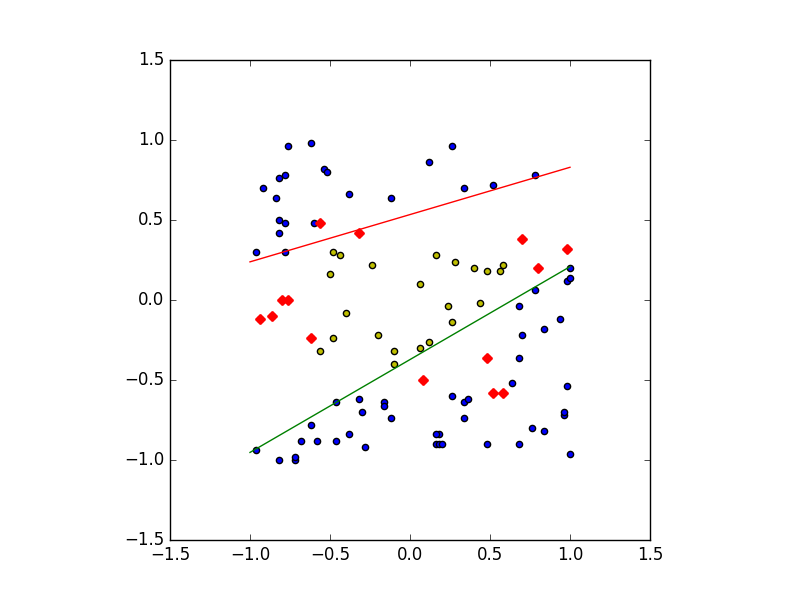
\includegraphics[width=\textwidth]{RecData-1HP.png}
    \caption{}
    \label{fig:RecData-1HP}
  \end{minipage}
  \hfill

Rectangle data trained with a single boundary hunter
\end{figure}

Figure \ref{fig:RecData-2HP} shows a Hyperplane GN Network with two boundary hunters trained on the same data. The hyperplanes align them selves with the rectangle boundary, showing that there is collaboration between the boundary hunters. If there was no cooperation then figure \ref{fig:RecData-1HP} would be equivalent to figure \ref{fig:RecData-2HP} with a boundary hunter removed.

\begin{figure}[H]
  \centering
  \begin{minipage}[b]{0.8\textwidth}
    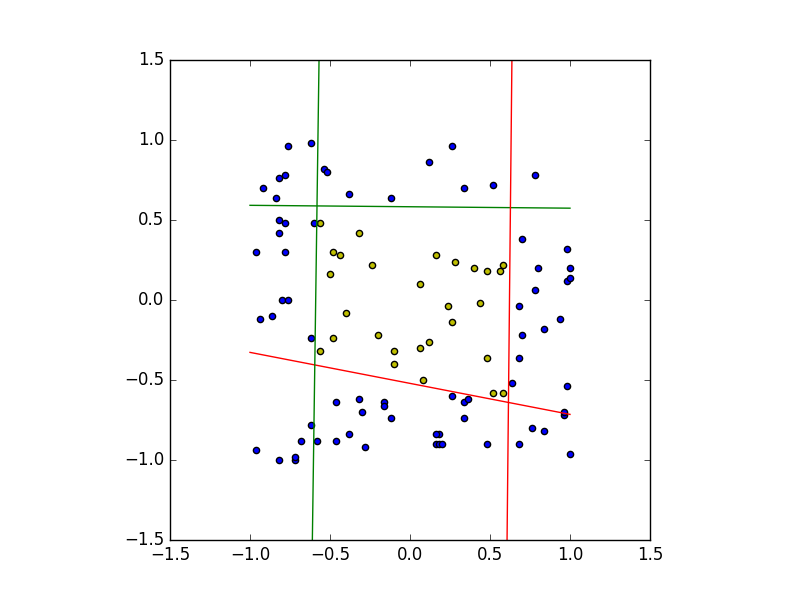
\includegraphics[width=\textwidth]{RecData-2HP.png}
    \caption{}
    \label{fig:RecData-2HP}
  \end{minipage}
  \hfill

Rectangle data trained with two boundary hunter
\end{figure}

Training these Hyperplane GN's individually would have no dependency between the boundary hunters but how will this effect the performance?

\chapter{Individual Hyperplane Gated Neurons}
Can hyperplane gated neurons be trained individually and achieve similar results to when they are trained in a network. Consider the loss when using the cross entropy error function.

\begin{align*}
	L = -\sum_{n=0}^N t_n log(\widehat{t_n}) + (1 - t_n) log(1 - \widehat{t_n})
\end{align*}

For a specific example $i$, without loss of generality say $t_n = 1$, then $l_i = log(\widehat{t_n}) = log(\sigma(\sigma(m \cdot x) \cdot (n \cdot x)))$ which can be simplified by substituting $r = \sigma(m \cdot x)$, resulting with $l_i = log(\sigma(r \cdot (n \cdot x)))$. As $r \rightarrow 0$, $l_i \rightarrow log(\frac{1}{2})$, so L is equivalent to equation \ref{equ:loss1}.\\

Consequently it is not surprising to see that training this set-up has the same results as section \ref{sec:lossfunction-a1}, figure \ref{fig:CHEVData-SingleBH} demonstrates this. \\

\begin{figure}[H]
  \centering
  \begin{minipage}[b]{0.8\textwidth}
    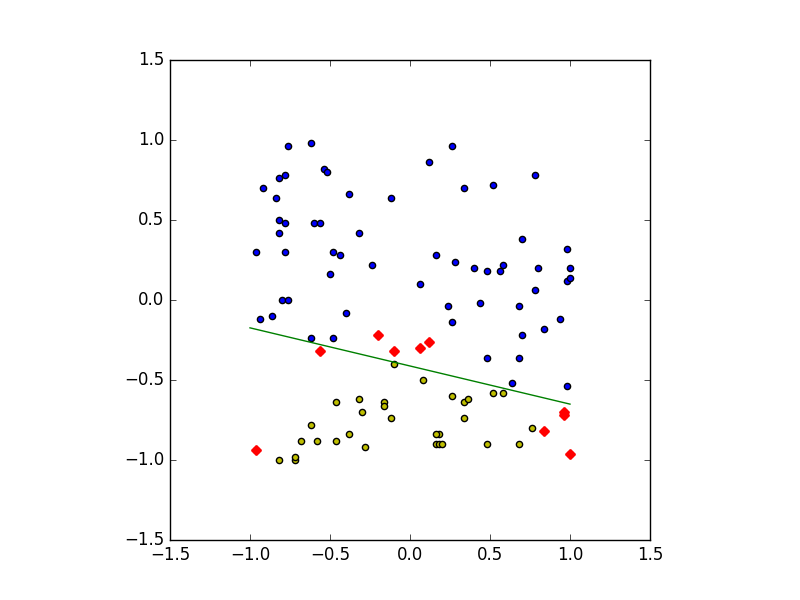
\includegraphics[width=\textwidth]{CHEVData-SingleBH.png}
    \caption{}
    \label{fig:CHEVData-SingleBH}
  \end{minipage}
  \hfill

Chevron data trained with a lone boundary hunter
\end{figure}

\section{Biases}
As the responsibility for example $i$ approaches 0 $\widehat{t_i} \rightarrow \frac{1}{2}$. $\widehat{t_i}$ represents the probability that example $i$ has a class of 1, when $\widehat{t_i} = \frac{1}{2}$ then it means that it is equally likely the true class to be 1 or 0. It is more likely that the probability of drawing an example with class 1 is not $\frac{1}{2}$.\\

Say probability of drawing a class 1 example which the boundary hunter does not care about is $p^c_1$. The loss over all examples which the boundary hunter is not responsible for is

\begin{align*}
	L_c &= -(n_1log(p_1) + n_0log(1-p_1))\\
	&= -(log(p_1^{n_1}) + log((1-p_1)^{n_0}))\\
	&= -(log(p_1^{n_1}(1-p_1)^{n_0}))
\end{align*}

where $n_a$ is the number of do not care examples of class $a$. Regardless of $n_0, n_1$ $p_1^{n_1}(1-p_1)^{n_0}$ has maximum value at $p_1 = \frac{1}{2}$ consequently $L_c$ also attains maximum value.

\begin{align}
	-log(p_1^{n_1}(1-p_1)^{n_0}) \leq -log(\frac{1}{2}^{n_1}\frac{1}{2}^{n_0})
	\label{equ:bias-comparason}
\end{align} 

Equation \ref{equ:bias-comparason} demonstrates that using the true distribution of the do not care data will give a lower loss. Consequently it makes more sense for a boundary hunter to learn the value which they output in the case they don't care. This parameter will be called bias $\beta$. 

\theoremstyle{definition}
\begin{definition}
	A \textbf{Hyperplane Gated Neuron with Bias} has the same parameters as the same parameters as a Hyperplane GN with an added bias $\beta$. Similarly to before $g = \sigma(m \cdot (c - x))$ and $f = n \cdot (c - x)$. Equation \ref{hyperplane-gated-neuron-bias-loss} defines the activation of this neuron.
	
	\begin{align}
	a(x) = \sigma(g(x) \cdot f(x) + (1 - g(x)) \cdot \beta)
	\label{hyperplane-gated-neuron-bias-loss}
	\end{align}
\end{definition}

Figure \ref{fig:CHEVData-SingleBH-WithByas} shows a Hyperplane GN with Bias trained on the chevron data, the result is the same that was achieved with a single neuron Hyperplane GN Network. 

\begin{figure}[H]
  \centering
  \begin{minipage}[b]{0.8\textwidth}
    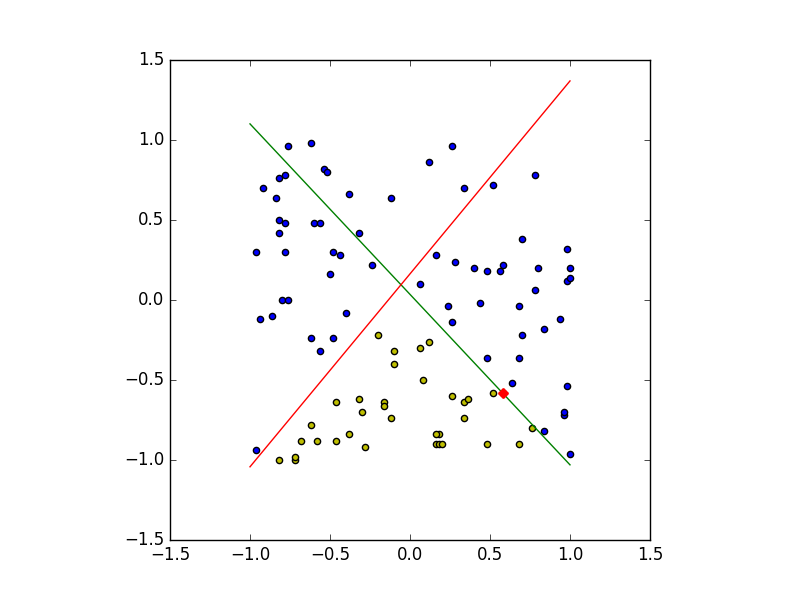
\includegraphics[width=\textwidth]{CHEVData-SingleBH-WithByas.png}
    \caption{}
    \label{fig:CHEVData-SingleBH-WithByas}
  \end{minipage}
  \hfill

Chevron data trained with a single boundary hunter that has a bias which is learnt.
\end{figure}

This is all very well but its very easy to learn the bias when the data has no noise. What would happen when training over the data in figure \ref{fig:noisychev-rawdata}

\begin{figure}[H]
  \centering
  \begin{minipage}[b]{0.8\textwidth}
    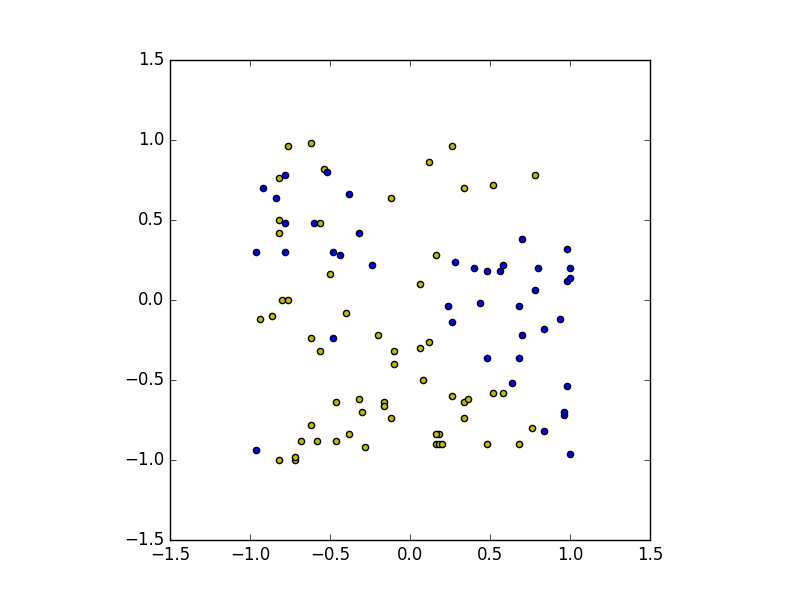
\includegraphics[width=\textwidth]{NoisyChev-RawData.png}
    \caption{}
    \label{fig:noisychev-rawdata}
  \end{minipage}
  \hfill
\end{figure}

With added noise the chevron becomes much less clear and could easily be interpreted in other ways, and while classifying the non noisy side of the chevron is still an option its not clear whether this is the best option. Figure \ref{fig:noisyChev-BH-withbias} shows that the boundary hunter is still able to identify the non noisy side of the chevron.

\begin{figure}[H]
  \centering
  \begin{minipage}[b]{0.8\textwidth}
    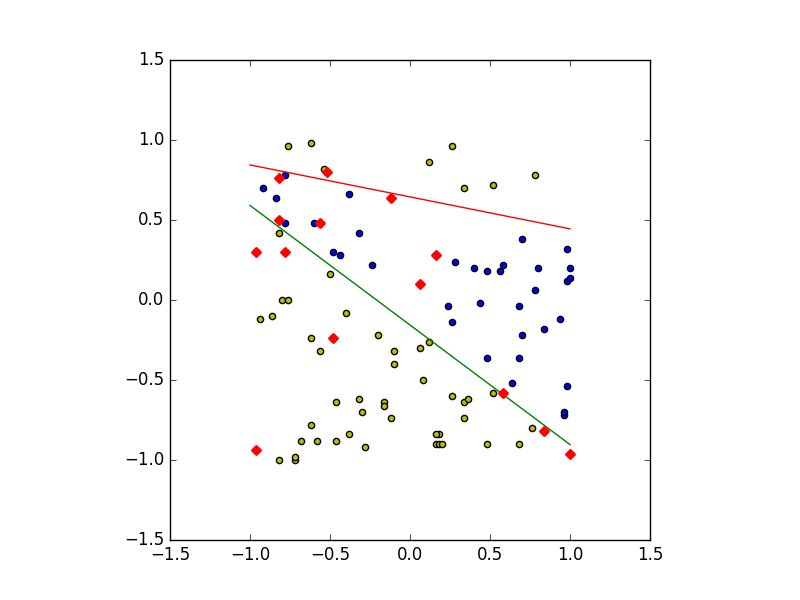
\includegraphics[width=\textwidth]{NoisyChev-BH-WithByas.png}
    \caption{}
    \label{fig:noisyChev-BH-withbias}
  \end{minipage}
  \hfill
\end{figure}
\chapter{Training in Higher Dimensions}
All testing up to this point has been performed in 2D, useful for visualisation but any real world problem will generally occupy a higher dimension. To test the Hyperplane BH in $n$ dimensions the vertices of an $n$ dimensional hypercube will be generated and divided up by two hyperplanes, representing the caring and decision boundaries. Then a Hyperplane BH will attempt to learn the generated boundaries.

\section{Results}
Until $n = 7$ the Hyperplane BH is able to perform at least as well as the generated solution, the data which on the do not care side of the data has a randomly assigned class so it might be possible to perform better than the generated solution. At $n = 7$ it no longer ignores all the data it should.\\

Any future work would first have to understand what is causing this issue. 

\chapter{Conclusion}
Locating local features in the data and ignoring everything else, a seemingly simple enough problem quickly became a difficult  balancing act of reward vs penalty. After attempting to design a loss which encouraged local learning we concluded that this was not a promising avenue to follow.\\

Using the idea of RBF Networks we where able to develop similar models of boundary hunters but this was not quite solving the problem we had in mind, the network structure meant there was some dependency between the hidden neurons. Removing the network and individually training these boundary hunter neurons did not initially have the results we wanted, after adding biases which where learned along side the weights we started to see the boundary hunters learning local features. Some tests on simple noisy data also proved promising.\\

Testing in higher dimensions revealed problems which where not seen on the 2D toy examples. Learning boundary hunters becomes difficult for $n > 7$. Consqeuently one remaining question is, what causes the diffcultys in learning when the number of dimentions increases?

This report has demonstrated that the concept of a boundary hunter is plausible but while there is difficulty learning in higher dimensions they can not be used in practice.


\newpage
\bibliographystyle{acm}
\bibliography{references}

\end{document}
